\documentclass[12pt,a4paper,spanish,oneside]{report}
\usepackage[T1]{fontenc}
\usepackage[utf8]{inputenc}
\usepackage[spanish]{babel}
\usepackage{graphicx}
\usepackage{booktabs}
\usepackage{array}
\usepackage{longtable}
\usepackage{geometry}
\usepackage{fancyhdr}
\usepackage{hyperref}
\usepackage{xcolor}
\usepackage{listings}
\usepackage{float}
\usepackage{tikz}
\usepackage{amssymb}
\usepackage{setspace}
\usepackage{parskip}

\graphicspath{{images/}}

\geometry{left=2.5cm,right=2.5cm,top=2.5cm,bottom=2.5cm}
\setlength{\headheight}{14.5pt}
\pagestyle{fancy}
\fancyhf{}
\rhead{\thepage}
\lhead{\textit{Sistema de Gestión de Agencias de K-Pop}}
\cfoot{\small Informe Técnico - K-POP World \textbf{V2.0}}

\lstset{
    language=bash,
    basicstyle=\ttfamily\small,
    breaklines=true,
    showstringspaces=false,
    keywordstyle=\color{blue},
    commentstyle=\color{gray},
    stringstyle=\color{red},
    escapeinside={(*}{*)},
    frame=tlrb,
    frameround=tttt,
    framesep=5pt
}

\title{\textbf{INFORME TÉCNICO} \\[0.5cm] \Large Sistema de Gestión de Agencias de K-Pop}
\author{Equipo de Desarrollo}
\date{16 de Enero de 2026 \\ Versión 2.0}

\begin{document}

% Portada personalizada
\begin{titlepage}
    \centering
    \vspace*{0.5cm}
    
    {\fontsize{26}{31}\selectfont \textbf{INFORME TÉCNICO}}
    
    \vspace{1cm}
    
    {\fontsize{28}{33}\selectfont \textbf{K-POP World}}
    
    \vspace{1.5cm}
    
    % Logo de la aplicación
    
\includegraphics[width=0.35\textwidth]{../KPopWorld logo.png}
    
    \vspace{1.5cm}
    
    {\Large \textcolor{gray}{Sistema de Gestión de Agencias de K-Pop}}
    
    \vspace{0.5cm}
    
    \vspace{2cm}
    
    
    {\normalsize \textbf{Equipo \#1}}
    
    \vspace{0.5cm}
    
    \begin{tabular}{lcr}
    \textit{Ronald Provance Valladares} & C-312 & @Ron\_1301 \\
    \textit{Agustín Alberto Carbajal Romero} & C-312 & @lil\_agus03 \\
    \textit{Daniel Amaranto Mares García} & C-312 & @amarantomc \\
    \textit{Dylan Ramsés Cabrera Morales} & C-312 & @dylan2108 \\
    \textit{Sheila Roque Alemán} & C-312 & @Luminara03 \\
    \end{tabular}
    
    \vspace{3cm}
    
    \vfill
    
    \vspace{0.5cm}
    
\end{titlepage}

\newpage

\tableofcontents
\newpage

\chapter{Introducción}

El presente informe técnico describe el diseño, modelado e implementación de un
sistema de información orientado a la gestión integral de agencias y grupos de K-pop. El
sistema fue desarrollado como parte del curso Bases de Datos II, aplicando principios de
modelado conceptual avanzado y arquitectura de software.
El objetivo principal del sistema es administrar de manera estructurada la información relacionada con agencias de entretenimiento, aprendices, artistas, grupos musicales,
actividades, contratos y evaluaciones, considerando relaciones complejas,
dependencias temporales y restricciones de integridad propias del dominio.
Para el diseño de la solución se empleó un Modelo Entidad–Relación Extendido (MERX),
el cual permitió representar especializaciones, relaciones históricas y entidades relacionales. Asimismo, se adoptó el enfoque de Clean Architecture con el fin de garantizar un alto
nivel de desacoplamiento, mantenibilidad y escalabilidad.
Este documento presenta el diccionario de datos, el esquema de clases, el diseño arquitectónico, la descripción del MERX final, la solución propuesta y las consideraciones
necesarias para el mantenimiento y evolución futura del sistema.

\chapter{Diccionario de Datos}

\section{Introducción}

El Diccionario de Datos es una referencia completa de todos los campos, tipos de datos y restricciones de cada tabla en la base de datos. Esta sección es esencial para desarrolladores y administradores de base de datos que realicen mantenimiento del sistema.

\section{Tabla: User}
La entidad User representa a los usuarios del sistema. Permite gestionar autenticación,
autorización y asociación con los distintos roles disponibles (admin, manager, director, aprendiz
y artista).
\begin{table}[H]
\centering
\caption{Diccionario - Tabla User}
\begin{tabular}{|l|l|l|l|l|}
\hline
\textbf{Campo} & \textbf{Tipo de Dato} & \textbf{Restricción} & \textbf{Descripción} \\
\hline
id & INTEGER & PK & Identificador único del usuario \\
\hline
email & VARCHAR & UNIQUE, NOT NULL & Correo electrónico \\
\hline
nombre & VARCHAR & NOT NULL & Nombre del usuario \\
\hline
password & VARCHAR & NOT NULL & Contraseña hasheada \\
\hline
rol & VARCHAR & NOT NULL & Rol en el sistema \\
\hline
\end{tabular}
\end{table}

\section{Tabla: PerfilManager}
Representa la especialización del usuario con rol de manager, asociado a una agencia
específica.
\begin{table}[H]
\centering
\caption{Diccionario - Tabla PerfilManager}
\begin{tabular}{|l|l|l|l|l|}
\hline
\textbf{Campo} & \textbf{Tipo de Dato} & \textbf{Restricción} & \textbf{Descripción} \\
\hline
userid & INTEGER & PK, FK(User)& Usuario asociado \\
\hline
agenciaId & INTEGER & FK(Agencia)& Agencia gestionada \\
\hline
\end{tabular}
\end{table}

\section{Tabla: PerfilDirector}
Representa la especialización del usuario con rol de director de una agencia.
\begin{table}[H]
\centering
\caption{Diccionario - Tabla PerfilDirector}
\begin{tabular}{|l|l|l|l|l|}
\hline
\textbf{Campo} & \textbf{Tipo de Dato} & \textbf{Restricción} & \textbf{Descripción} \\
\hline
userid & INTEGER & PK, FK(User)& Usuario asociado \\
\hline
agenciaId & INTEGER & FK(Agencia)& Agencia dirigida \\
\hline
\end{tabular}
\end{table}

\section{Tabla: PerfilAprendiz}
Asocia un usuario con un aprendiz del sistema
\begin{table}[H]
\centering
\caption{Diccionario - Tabla PerfilAprendiz}
\begin{tabular}{|l|l|l|l|l|}
\hline
\textbf{Campo} & \textbf{Tipo de Dato} & \textbf{Restricción} & \textbf{Descripción} \\
\hline
userid & INTEGER & PK, FK(User)& Usuario asociado \\
\hline
aprendizId & INTEGER & FK(Aprendiz)& Aprendiz vinculado \\
\hline
\end{tabular}
\end{table}

\section{Tabla: PerfilArtista}
Relaciona un usuario con un artista, considerando su pertenencia a un grupo.
\begin{table}[H]
\centering
\caption{Diccionario - Tabla PerfilArtista}
\begin{tabular}{|l|l|l|l|l|}
\hline
\textbf{Campo} & \textbf{Tipo de Dato} & \textbf{Restricción} & \textbf{Descripción} \\
\hline
userid & INTEGER & PK, FK(User)& Usuario asociado \\
\hline
IdAp & INTEGER & FK(Aprendiz)& Identificador del aprendiz \\
\hline
IdGr & INTEGER & FK(Grupo) & Grupo de Debut del artista \\
\hline
\end{tabular}
\end{table}

\section{Tabla: Agencia}
La entidad Agencia representa a las compañías de entretenimiento responsables de
la gestión de aprendices, artistas y grupos musicales. Una agencia puede administrar
múltiples grupos, contratos, evaluaciones y solicitudes, actuando como eje central del
sistema.

\begin{table}[H]
\centering
\caption{Diccionario - Tabla Agencia}
\begin{tabular}{|l|l|l|l|l|}
\hline
\textbf{Campo} & \textbf{Tipo de Dato} & \textbf{Restricción} & \textbf{Descripción} \\
\hline
id & INTEGER & PK & Identificador único de la agencia \\
\hline
nombre & VARCHAR & NOT NULL & Nombre oficial de la agencia \\
\hline
ubicacion & VARCHAR & NOT NULL & Ubicación geográfica \\
\hline
fechaFundacion & DATE & NOT NULL & Fecha de fundación \\
\hline
\end{tabular}
\end{table}

\section{Tabla: Aprendiz}
La entidad Aprendiz representa a una persona en proceso de formación dentro de una agencia.
\begin{table}[H]
\centering
\caption{Diccionario - Tabla Aprendiz}
\begin{tabular}{|l|l|l|l|l|}
\hline
\textbf{Campo} & \textbf{Tipo de Dato}  & \textbf{Restricción} & \textbf{Descripción} \\
\hline
id & INTEGER & PK & Identificador único del aprendiz \\
\hline
idSolicitud & INTEGER & FK(Solicitud) & Identificador de la solicitud \\
\hline
nombreCompleto & VARCHAR & NOT NULL & Nombre completo \\
\hline
fechaNacimiento & DATE & NOT NULL & Fecha de nacimiento \\
\hline
edad & INTEGER & NOT NULL & Edad del aprendiz \\
\hline
nivelEntrenamiento & INTEGER & NOT NULL & Nivel de Entrenamiento \\
\hline
\end{tabular}
\end{table}

\section{Tabla: Grupo}
La entidad Grupo representa un conjunto de artistas que desarrollan actividades mu-
sicales de manera conjunta. Cada grupo se encuentra asociado a una agencia, un concepto
artístico y un concepto visual, y mantiene información histórica sobre sus integrantes, ac-
tividades, lanzamientos y contratos.

\begin{table}[H]
\centering
\caption{Diccionario - Tabla Grupo}
\begin{tabular}{|l|l|l|l|l|}
\hline
\textbf{Campo} & \textbf{Tipo de Dato} & \textbf{Restricción} & \textbf{Descripción} \\
\hline
id & INTEGER & PK & Identificador único \\
\hline
nombreCompleto & VARCHAR & NOT NULL & Nombre del grupo \\
\hline
fechaDebut & DATE & NOT NULL & Fecha oficial de debut \\
\hline
estadoGrupo & VARCHAR & NOT NULL & Estado actual del grupo \\
\hline
idConcepto & INTEGER & FK(Concepto) & Concepto artístico asociado \\
\hline
idConceptoVisual & INTEGER & FK(ConceptoVisual) & Concepto visual asociado \\
\hline
Nomiembros & INTEGER & NOT NULL & Cantidad de miembros \\
\hline
\end{tabular}
\end{table}

\section{Tabla: Artista}
La entidad Artista representa a un aprendiz que ha debutado oficialmente en la
industria musical. Un artista puede formar parte de uno o varios grupos a lo largo de su
carrera o desempeñarse como solista durante determinados períodos de tiempo.
\begin{table}[H]
\centering
\caption{Diccionario - Tabla Artista}
\begin{tabular}{|l|l|l|l|l|}
\hline
\textbf{Campo} & \textbf{Tipo de Dato} & \textbf{Restricción} & \textbf{Descripción} \\
\hline
idAp & INTEGER & PK,FK(Aprendiz) & Identificador del aprendiz\\
\hline
idGr & INTEGER & PK,FK(Grupo) & Grupo de debut del artista \\
\hline
idSolicitud & INTEGER & FK(Solicitud) & Identificador de la solicitud \\
\hline
nombreArtistico & VARCHAR & NOT NULL & Nombre artístico \\
\hline
fechaDebut & DATE & NOT NULL & Fecha de debut oficial \\
\hline
estadoArtista & VARCHAR & NOT NULL & Estado actual del artista \\
\hline
\end{tabular}
\end{table}
\section{Tabla: Concepto}
La entidad Concepto representa el estilo artístico general de un grupo musical.
\begin{table}[H]
\centering
\caption{Diccionario - Tabla Concepto}


\begin{tabular}{|l|l|l|l|l|}
\hline
\textbf{Campo} & \textbf{Tipo de Dato} & \textbf{Restricción} & \textbf{Descripción} \\
\hline
id & INTEGER & PK & Identificador del concepto \\
\hline
nombre & VARCHAR & NOT NULL & Nombre del concepto \\
\hline
descripcion & VARCHAR & NOT NULL & Descripción del concepto \\
\hline
\end{tabular}
\end{table}

\section{Tabla: Concepto Visual}
La entidad ConceptoVisual representa la identidad visual exclusiva de un grupo musical
\begin{table}[H]
\centering
\caption{Diccionario - Tabla Concepto Visual}


\begin{tabular}{|l|l|l|l|l|}
\hline
\textbf{Campo} & \textbf{Tipo de Dato} & \textbf{Restricción} & \textbf{Descripción} \\
\hline
id & INTEGER & PK & Identificador del concepto visual\\
\hline
imagen & VARCHAR & NOT NULL & Imagen representativa del concepto visual \\
\hline
\end{tabular}
\end{table}

\section{Tabla: Álbum}
La entidad Álbum representa una producción musical lanzada por un grupo y/o artistas. Contiene información relacionada con el lanzamiento, producción, ventas y relaciones con canciones, premios y participantes.
\begin{table}[H]
\centering
\caption{Diccionario - Tabla Álbum}
\begin{tabular}{|l|l|l|l|l|}
\hline
\textbf{Campo} & \textbf{Tipo de Dato} & \textbf{Restricción} & \textbf{Descripción} \\
\hline
id & INTEGER & PK & Identificador del álbum \\
\hline
titulo & VARCHAR & NOT NULL & Título del álbum \\
\hline
fechaLanzamiento & DATE & NOT NULL & Fecha de lanzamiento \\
\hline
productor & VARCHAR & NOT NULL & Productor musical del álbum \\
\hline
NoCanciones & INTEGER & NOT NULL & Número de canciones \\
\hline
NoCopiasVendidas & INTEGER & NOT NULL & Copias vendidas \\
\hline
\end{tabular}
\end{table}

\section{Tabla: Canción}
La entidad Canción representa una composición musical que forma parte de uno o varios álbumes y puede posicionarse en listas de popularidad.
\begin{table}[H]
\centering
\caption{Diccionario - Tabla Canción}
\begin{tabular}{|l|l|l|l|l|}
\hline
\textbf{Campo} & \textbf{Tipo de Dato} & \textbf{Restricción} & \textbf{Descripción} \\
\hline
id & INTEGER & PK & Identificador de la canción \\
\hline
titulo & VARCHAR & NOT NULL & Título de la canción \\
\hline
genero & VARCHAR & NOT NULL & Género musical \\
\hline
productor & VARCHAR & NOT NULL & Productor de la canción \\
\hline
fechaLanzamiento & DATE & NOT NULL & Fecha de lanzamiento \\
\hline
reproducciones & INTEGER & NOT NULL & Cantidad de reproducciones \\
\hline
\end{tabular}
\end{table}

\section{Tabla: Lista de Popularidad}
La entidad ListaPopularidad representa los rankings musicales nacionales o internacionales en los que se posicionan las canciones, permitiendo registrar históricamente su desempeño a lo largo del tiempo.
\begin{table}[H]
\centering
\caption{Diccionario - Tabla Lista de Popularidad}
\begin{tabular}{|l|l|l|l|l|}
\hline
\textbf{Campo} & \textbf{Tipo de Dato} & \textbf{Restricción} & \textbf{Descripción} \\
\hline
id & INTEGER & PK & Identificador de la lista \\
\hline
nombre & VARCHAR & NOT NULL & Nombre de la lista de popularidad \\
\hline
tipoLista & VARCHAR & NOT NULL & Tipo de Lista \\
\hline
requisito & INTEGER & NOT NULL & Requisito para posicionarse en la lista \\
\hline
\end{tabular}
\end{table}

\section{Tabla: Actividad}
La entidad Actividad representa los eventos organizados por las agencias tales como conciertos, promociones, sesiones de grabación u otros eventos relacionados con la industria musical. Cada actividad puede generar ingresos y contar con la
participación de artistas y grupos.
\begin{table}[H]
\centering
\caption{Diccionario - Tabla Actividad}
\begin{tabular}{|l|l|l|l|l|}
\hline
\textbf{Campo} & \textbf{Tipo de Dato} & \textbf{Restricción} & \textbf{Descripción} \\
\hline
id & INTEGER  & PK & Identificador único de la actividad \\
\hline
responsable & VARCHAR & NOT NULL & Responsable de la actividad \\
\hline
lugar & VARCHAR & NOT NULL & Ubicación de la actividad  \\
\hline
fecha & DATE & NOT NULL & Fecha de realización de la actividad \\
\hline
tipoActividad & VARCHAR & NOT NULL & Tipo de actividad \\
\hline
tipoEvento & VARCHAR & NOT NULL & Tipo de evento \\
\hline
estado & VARCHAR & NOT NULL & Estado de la actividad \\
\hline
\end{tabular}
\end{table}

\section{Tabla: Premio}
La entidad Premio representa los reconocimientos otorgados por academias o instituciones musicales a producciones destacadas.
\begin{table}[H]
\centering
\caption{Diccionario - Tabla Premio}
\begin{tabular}{|l|l|l|l|l|}
\hline
\textbf{Campo} & \textbf{Tipo de Dato} & \textbf{Restricción} & \textbf{Descripción} \\
\hline
id & INTEGER & PK & Identificador único del premio \\
\hline
tituloPremio & VARCHAR & NOT NULL & Nombre del premio otorgado\\
\hline
nombreAcademia & VARCHAR & NOT NULL & Academia o institución otorgante \\
\hline
requisito & INTEGER & NOT NULL & Requisito para obtener el premio \\
\hline
\end{tabular}
\end{table}

\section{Tabla: Ingreso}
La entidad Ingreso registra los beneficios económicos obtenidos como resultado de una actividad específica, permitiendo llevar un control financiero del sistema
\begin{table}[H]
\centering
\caption{Diccionario - Tabla Ingreso}
\begin{tabular}{|l|l|l|l|l|}
\hline
\textbf{Campo} & \textbf{Tipo de Dato} & \textbf{Restricción} & \textbf{Descripción} \\
\hline
idIng & INTEGER & PK & Identificador del ingreso \\
\hline
idAct & INTEGER & PK,FK(Actividad)& Actividad asociada \\
\hline
monto & DECIMAL & NOT NULL & Monto del ingreso \\
\hline
fecha & DATE & NOT NULL & Fecha del ingreso \\
\hline
descripcion & VARCHAR & NOT NULL & Descripción del ingreso \\
\hline
\end{tabular}
\end{table}

\section{Tabla: Solicitud}
La entidad Solicitud representa una propuesta formal para la creación o integración a
un grupo musical. Dicha solicitud puede involucrar tanto aprendices como artistas activos
y es gestionada por una agencia.
\begin{table}[H]
\centering
\caption{Diccionario - Tabla Solicitud}
\begin{tabular}{|l|l|l|l|l|}
\hline
\textbf{Campo} & \textbf{Tipo de Dato} & \textbf{Restricción} & \textbf{Descripción} \\
\hline
id & INTEGER & PK & Identificador de la solicitud \\
\hline
nombreGrupo & VARCHAR & NOT NULL & Nombre propuesto para el grupo \\
\hline
idConcepto & INTEGER & FK(Concepto) & Concepto propuesto para el grupo \\
\hline
idAgencia & INTEGER & FK(Agencia) & Agencia que gestiona la solicitud \\
\hline
fechaSolicitud & DATE & NOT NULL & Fecha de la solicitud \\
\hline
estado & VARCHAR & NOT NULL & Estado actual de la solicitud \\
\hline
\end{tabular}
\end{table}

\section{Tabla: Contrato}
La entidad Contrato representa los acuerdos contractuales establecidos entre una
agencia y un artista. Dichos contratos regulan las condiciones bajo las cuales el artista
desarrolla actividades profesionales bajo la gestión de una agencia.
\begin{table}[H]
\centering
\caption{Diccionario - Tabla Contrato}
\begin{tabular}{|l|l|l|l|l|}
\hline
\textbf{Campo} & \textbf{Tipo de Dato} & \textbf{Restricción} & \textbf{Descripción} \\
\hline
idAg & INTEGER & PK,FK(Agencia) & Identificador de la agencia \\
\hline
idAp & INTEGER & PK,FK(Artista) & Identificador del aprendiz \\
\hline
idGr & INTEGER & PK,FK(Artista) & Identificador del grupo  \\
\hline
fechaInicio & DATE & PK & Fecha de inicio del contrato \\
\hline
fechaFinalizacion & DATE & NOT NULL & Fecha de finalización del contrato \\
\hline
estado & VARCHAR & NOT NULL & Estado actual del contrato \\
\hline
condicionesIniciales & VARCHAR & NOT NULL & Condiciones iniciales del contrato \\
\hline
distribucionIngresos & VARCHAR & NOT NULL & Distribución de ingresos acordada \\
\hline
\end{tabular}
\end{table}

\section{Tabla: ContratoGrupo}
La entidad ContratoGrupo representa los acuerdos contractuales establecidos entre una
agencia y un grupo.
\begin{table}[H]
\centering
\caption{Diccionario - Tabla ContratoGrupo}
\begin{tabular}{|l|l|l|l|l|}
\hline
\textbf{Campo} & \textbf{Tipo de Dato} & \textbf{Restricción} & \textbf{Descripción} \\
\hline
id & INTEGER & PK & Identificador del contrato \\
\hline
idAg & INTEGER & FK(Agencia) & Identificador de la agencia \\
\hline
idGr & INTEGER & FK(Artista) & Identificador del grupo  \\
\hline
fechaInicio & DATE & PK & Fecha de inicio del contrato \\
\hline
fechaFinalizacion & DATE & NOT NULL & Fecha de finalización del contrato \\
\hline
estado & VARCHAR & NOT NULL & Estado actual del contrato \\
\hline
condicionesIniciales & VARCHAR & NOT NULL & Condiciones iniciales del contrato \\
\hline
distribucionIngresos & VARCHAR & NOT NULL & Distribución de ingresos acordada \\
\hline
\end{tabular}
\end{table}

\section{Tabla: ArtistaEnGrupo}
La entidad ArtistaEnGrupo registra la pertenencia histórica de un artista a un grupo
musical, permitiendo modelar cambios de alineación a lo largo del tiempo y preservar
información temporal.
\begin{table}[H]
\centering
\caption{Diccionario - Tabla ArtistaEnGrupo}
\begin{tabular}{|l|l|l|l|l|}
\hline
\textbf{Campo} & \textbf{Tipo de Dato} & \textbf{Restricción} & \textbf{Descripción} \\
\hline
idAp & INTEGER & PK,FK(Artista) & Identificador del artista \\
\hline
idGrupoDebut & INTEGER & PK,FK(Artista) & Identificador del grupo de debut  \\
\hline
idGr & INTEGER & PK,FK(Grupo) & Identificador del grupo  \\
\hline
fechaInicio & DATE & PK & Fecha de inicio en grupo \\
\hline
fechaFinalizacion & DATE & NOT NULL & Fecha de finalización en grupo \\
\hline
rol & VARCHAR & NOT NULL & Rol del artista en el grupo \\
\hline
\end{tabular}
\end{table}

\section{Tabla: AlbumPremiado}
La entidad AlbumPremiado relaciona álbums con los premios que han recibido,
permitiendo registrar el año en que se otorgó cada reconocimiento.
\begin{table}[H]
\centering
\caption{Diccionario - Tabla AlbumPremiado}
\begin{tabular}{|l|l|l|l|l|}
\hline
\textbf{Campo} & \textbf{Tipo de Dato} & \textbf{Restricción} & \textbf{Descripción} \\
\hline
idAlb & INTEGER & PK,FK(Album) & Identificador del álbum \\
\hline
idPremio & INTEGER & PK,FK(Premio) & Identificador del premio \\
\hline
año & INTEGER & NOT NULL & Año en que se otorgó el premio \\
\hline
\end{tabular}
\end{table}

\section{Tabla: CancionEnListaDePopularidad}
La entidad CancionEnListaDePopularidad registra la posición histórica de una
canción dentro de una lista de popularidad en un año determinado.
\begin{table}[H]
\centering
\caption{Diccionario - Tabla CancionEnListaDePopularidad}
\begin{tabular}{|l|l|l|l|l|}
\hline
\textbf{Campo} & \textbf{Tipo de Dato} & \textbf{Restricción} & \textbf{Descripción} \\
\hline
idCa & INTEGER & PK,FK(Cancion) & Identificador de la canción \\
\hline
idLista & INTEGER & PK,FK(ListaPopularidad) & Identificador de la lista de popularidad \\
\hline
posicion & INTEGER & NOT NULL & Posición alcanzada en la lista \\
año & INTEGER & NOT NULL & Año del ranking \\
\hline
\end{tabular}
\end{table}

\section{Tabla: AprendizEnAgencia}
La entidad AprendizEnAgencia registra la relación temporal entre un aprendiz y
una agencia, permitiendo conservar el historial de permanencia del aprendiz.
\begin{table}[H]
\centering
\caption{Diccionario - Tabla AprendizEnAgencia}
\begin{tabular}{|l|l|l|l|l|}
\hline
\textbf{Campo} & \textbf{Tipo de Dato} & \textbf{Restricción} & \textbf{Descripción} \\
\hline
idAp & INTEGER & PK,FK(Aprendiz) & Identificador del aprendiz \\
\hline
idAg & INTEGER & PK,FK(Agencia) & Identificador de la agencia \\
\hline
fechaInicio & DATE & PK & Fecha de inicio en la agencia \\
\hline
fechaFinalizacion & DATE & NOT NULL & Fecha de finalización en la agencia \\
\hline
estado & VARCHAR & NOT NULL & Estado del aprendiz en la agencia \\
\hline
\end{tabular}
\end{table}

\section{Tabla: EvaluacionAprendiz}
La entidad EvaluacionAprendiz registra las evaluaciones periódicas realizadas a los aprendices por parte de las agencias.
\begin{table}[H]
\centering
\caption{Diccionario - Tabla EvaluacionAprendiz}
\begin{tabular}{|l|l|l|l|l|}
\hline
\textbf{Campo} & \textbf{Tipo de Dato} & \textbf{Restricción} & \textbf{Descripción} \\
\hline
idAp & INTEGER & PK,FK(Aprendiz) & Identificador del aprendiz \\
\hline
idAg & INTEGER & PK,FK(Agencia) & Identificador de la agencia \\
\hline
fechaEvaluacion & DATE & PK & Fecha de evaluación \\
\hline
evaluacion & INTEGER & NOT NULL & Resultado de la evaluación\\
\hline
\end{tabular}
\end{table}

\section{Tabla: PersonasEnActividad}
La entidad PersonasEnActividad registra la participación de artistas o grupos en
una actividad específica, indicando si dicha participación fue aprobada.
\begin{table}[H]
\centering
\caption{Diccionario - Tabla PersonasEnActividad}
\begin{tabular}{|l|l|l|l|l|}
\hline
\textbf{Campo} & \textbf{Tipo de Dato} & \textbf{Restricción} & \textbf{Descripción} \\
\hline
id & INTEGER & PK & Identificador de la participación\\
\hline
idAp & INTEGER & FK(Artista) & Artista participante \\
\hline
idGr & INTEGER & FK(Artista) & Grupo de debut del artista \\
\hline
idAct & INTEGER & FK(Actividad) & Actividad asociada\\
\hline
idGrupos & INTEGER & FK(Grupo) & Grupo participante \\
\hline
aceptado & BOOLEAN & NULLABLE & Indica si la participación fue aprobada \\
\hline
\end{tabular}
\end{table}

\section{Tabla: ArtistaLanzaAlbum}
La entidad ArtistaLanzaAlbum relaciona artistas con álbumes lanzados.
\begin{table}[H]
\centering
\caption{Diccionario - Tabla ArtistaLanzaAlbum}
\begin{tabular}{|l|l|l|l|l|}
\hline
\textbf{Campo} & \textbf{Tipo de Dato} & \textbf{Restricción} & \textbf{Descripción} \\
\hline
idAp & INTEGER & PK,FK(Artista) & Identificador del artista\\
\hline
idGr & INTEGER & PK,FK(Artista) & Grupo de debut del artista \\
\hline
idAlb & INTEGER & PK,FK(Album) & Identificador del álbum lanzado \\
\hline
\end{tabular}
\end{table}

\section{Tabla: GrupoLanzaAlbum}
La entidad GrupoLanzaAlbum relaciona grupos musicales con álbumes lanzados.
\begin{table}[H]
\centering
\caption{Diccionario - Tabla GrupoLanzaAlbum}
\begin{tabular}{|l|l|l|l|l|}
\hline
\textbf{Campo} & \textbf{Tipo de Dato} & \textbf{Restricción} & \textbf{Descripción} \\
\hline
idGr & INTEGER & PK,FK(Grupo) & Identificador del grupo \\
\hline
idAlb & INTEGER & PK,FK(Album) & Identificador del álbum lanzado \\
\hline
\end{tabular}
\end{table}

\section{Tabla: AprendizSolicitaGrupo}
La entidad AprendizSolicitaGrupo registra la participación de aprendices en solicitudes de creación de grupos musicales.
\begin{table}[H]
\centering
\caption{Diccionario - Tabla AprendizSolicitaGrupo}
\begin{tabular}{|l|l|l|l|l|}
\hline
\textbf{Campo} & \textbf{Tipo de Dato} & \textbf{Restricción} & \textbf{Descripción} \\
\hline
idAp & INTEGER & PK,FK(Aprendiz) & Aprendiz Solicitante \\
\hline
idAg & INTEGER & PK,FK(Agencia) & Agencia asociada \\
\hline
idSolicitud & INTEGER & PK,FK(Solicitud) & Solicitud asociada \\
\hline
estado & VARCHAR & NOT NULL & Estado de la solicitud \\
\hline
\end{tabular}
\end{table}

\section{Tabla: ArtistaSolicitaGrupo}
La entidad ArtistaSolicitaGrupo registra la participación de artistas en solicitudes de creación de grupos musicales.
\begin{table}[H]
\centering
\caption{Diccionario - Tabla AprendizSolicitaGrupo}
\begin{tabular}{|l|l|l|l|l|}
\hline
\textbf{Campo} & \textbf{Tipo de Dato} & \textbf{Restricción} & \textbf{Descripción} \\
\hline
idAp & INTEGER & PK,FK(Artista) & Artista Solicitante \\
\hline
idGr & INTEGER & PK,FK(Artista) & Grupo de debut del artista \\
\hline
idAg & INTEGER & PK,FK(Agencia) & Agencia asociada \\
\hline
idSolicitud & INTEGER & PK,FK(Solicitud) & Solicitud asociada \\
\hline
estado & VARCHAR & NOT NULL & Estado de la solicitud \\
\hline
\end{tabular}
\end{table}

\chapter{Diseño de la aplicación}
El sistema de gestión de agencias y grupos de K-pop fue diseñado siguiendo los principios de Clean Architecture, con el objetivo de garantizar un alto nivel de desacoplamiento, mantenibilidad, escalabilidad y facilidad de prueba.
Esta arquitectura permite separar claramente las responsabilidades del sistema, evitando dependencias directas entre la lógica de negocio y los detalles de infraestructura o presentación.
\section{Arquitectura general}
La arquitectura del sistema se organiza en capas concéntricas, donde las dependencias
siempre apuntan hacia el núcleo del sistema. Las capas principales son:
\begin{itemize}
    \item Capa de Dominio
    \item Capa de Aplicación
    \item Capa de Infraestructura
    \item Capa de Presentación
\end{itemize}
Cada capa cumple una función específica y se comunica con las demás mediante interfaces bien definidas.

\subsection{Capa de Dominio}
La capa de dominio constituye el núcleo del sistema. Contiene las entidades principales
del negocio, así como las reglas y restricciones fundamentales del dominio.
En esta capa se definen:
\begin{itemize}
    \item Entidades como Agencia, Aprendiz, Artista, Grupo, Álbum y Contrato.
    \item Reglas de negocio relacionadas con contratos, pertenencia a grupos y estados.
    \item Restricciones temporales y de integridad del dominio.
\end{itemize}
Esta capa no depende de ninguna tecnología externa ni de frameworks específicos.

\subsection{Capa de Aplicación}
La capa de aplicación orquesta los casos de uso del sistema y actúa como intermediaria
entre la capa de dominio y las capas externas. Sus responsabilidades incluyen:
\begin{itemize}
    \item Implementación de casos de uso como creación, eliminación, actualización y obtención de cada entidad, así como otros casos de gestión de la entidad.
    \item Coordinación de flujos de datos entre entidades.
    \item Validación de reglas de negocio complejas.
\end{itemize}
Esta capa depende únicamente de abstracciones definidas en el dominio.

\subsection{Capa de Infraestructura}
La capa de infraestructura contiene los detalles técnicos de implementación, incluyendo el acceso a datos y servicios externos. En esta capa se encuentran:
\begin{itemize}
    \item Implementación de repositorios mediante Prisma ORM.
    \item Conexión y persistencia de datos en PostgreSQL.
    \item Configuración de servicios externos y utilidades.
\end{itemize}
Esta capa implementa las interfaces definidas por la capa de aplicación.

\subsection{Capa de Presentación}
La capa de presentación expone la API HTTP y actúa como la interfaz entre los clientes (frontend) y la lógica de la aplicación. Se encarga de recibir peticiones, validar y normalizar datos de entrada, orquestar llamadas a los casos de uso y formatear las respuestas HTTP para el cliente. En esta capa se encuentran:
\begin{itemize}
    \item Controladores por recurso (por ejemplo GroupController, UserController): reciben Request/Response, usan DTOs para validar/transformar la entrada y delegan la ejecución a los Use Cases inyectados.
    \item Definición de rutas: clases que crean Routers y asignan endpoints (GET/POST/PUT/DELETE), agrupadas y montadas en el router raíz (routes/index.ts) con prefijos claros (/group, /auth, /user, ...).
    \item Uso de DTOs y validaciones: los controladores consumen DTOs desde la capa de aplicación para garantizar formato y reglas antes de invocar la lógica de negocio.
    \item Middlewares de presentación: autenticación y autorización (AuthMiddleware, RoleMiddleware) y otros pre-procesos que ejecutan antes de llegar a los controladores.
\end{itemize}

\section{Flujo de Datos}
El flujo de datos del sistema sigue el principio de inversión de dependencias. Las solicitudes del usuario se originan en la capa de presentación, pasan por la capa de aplicación
y afectan al dominio, mientras que la persistencia se realiza a través de la infraestructura.
Este enfoque permite que el sistema sea fácilmente extensible y adaptable a cambios
futuros en tecnologías o requerimientos.

\chapter{Esquema de clases}

El diseño de clases del sistema se estructura siguiendo los principios de la arquitectura limpia y está organizado en la capa de dominio. Las clases definidas representan las entidades principales del negocio, cada una con responsabilidades específicas y relaciones claramente definidas con otras entidades.

\section{Clases principales del dominio}

\subsection{Clase User (Usuario)}
Clase abstracta que representa a los usuarios del sistema. Define los atributos comunes a todos los usuarios y establece un contrato para que las clases derivadas implementen el método \texttt{getProfileData()}.

\begin{itemize}
	\item \textbf{Atributos:} id (identificador único), name (nombre), email (correo electrónico), password (contraseña), role (rol del usuario)
	\item \textbf{Relación:} Superclase de AdminUser, ManagerUser, DirectorUser, ApprenticeUser y ArtistUser
	\item \textbf{Responsabilidad:} Almacenar información común de autenticación y perfil de usuario
\end{itemize}

\subsection{Clase Agency (Agencia)}
Representa una agencia de entretenimiento en el sistema. Las agencias son la entidad raíz que agrupa a managers, directores, aprendices y artistas.

\begin{itemize}
	\item \textbf{Atributos:} id, name (nombre de la agencia), address (dirección), foundation (fecha de fundación)
	\item \textbf{Relaciones:} 
	\begin{itemize}
		\item Contiene múltiples Apprentice (aprendices)
		\item Contiene múltiples Group (grupos)
		\item Contiene múltiples ManagerUser y DirectorUser
		\item Participa en múltiples Contract (contratos)
	\end{itemize}
	\item \textbf{Responsabilidad:} Servir como contenedor y punto de control para la gestión de talento y recursos
\end{itemize}

\subsection{Clase Apprentice (Aprendiz)}
Representa a un aspirante a artista que se encuentra en formación dentro de una agencia.

\begin{itemize}
	\item \textbf{Atributos:} id, name (nombre), dateOfBirth (fecha de nacimiento), age (edad calculada), trainingLv (nivel de entrenamiento), status (estado actual del aprendiz)
	\item \textbf{Relaciones:}
	\begin{itemize}
		\item Pertenece a una Agency
		\item Puede formar parte de un Group
		\item Puede generar Album (cuando debuta)
		\item Puede participar en Activity (actividades)
		\item Tiene evaluaciones ApprenticeEvaluation
	\end{itemize}
	\item \textbf{Responsabilidad:} Representar la etapa inicial de formación de los artistas
\end{itemize}

\subsection{Clase Artist (Artista)}
Representa a un artista profesional que ha debutado en el sistema. Un artista es una evolución de un aprendiz que ha integrado un grupo.

\begin{itemize}
	\item \textbf{Atributos:} ApprenticeId (identificador del aprendiz original), GroupId (grupo actual), ArtistName (nombre artístico), DebutDate (fecha de debut), Status (estado: activo, inactivo, retirado), realName (nombre real), agencyId (identificador de agencia)
	\item \textbf{Atributo adicional:} GroupHistory (historial de grupos a los que ha pertenecido)
	\item \textbf{Relaciones:}
	\begin{itemize}
		\item Registra un Apprentice como antecedente
		\item Participa en uno o múltiples Group
		\item Participa en múltiples Activity
		\item Tiene múltiples Contract
		\item Genera Income (ingresos)
	\end{itemize}
	\item \textbf{Responsabilidad:} Representar la carrera profesional de un artista, con seguimiento de grupos y participaciones
\end{itemize}

\subsection{Clase Group (Grupo)}
Representa un grupo musical formado por uno o más artistas/aprendices bajo la supervisión de una agencia.

\begin{itemize}
	\item \textbf{Atributos:} id, name (nombre del grupo), debut (fecha de debut), status (estado: activo, disuelto, en pausa), memberCount (número de miembros), agency (agencia responsable), concept (concepto creativo), visualConcept (concepto visual)
	\item \textbf{Relaciones:}
	\begin{itemize}
		\item Pertenece a una Agency
		\item Asociado a un Concept (identidad creativa)
		\item Posee un VisualConcept (identidad visual única)
		\item Contiene múltiples miembros (artistas/aprendices)
		\item Genera múltiples Album
		\item Participa en múltiples Activity
		\item Tiene múltiples Contract
	\end{itemize}
	\item \textbf{Responsabilidad:} Agrupar artistas y gestionar su actividad colectiva
\end{itemize}

\subsection{Clase Contract (Contrato)}
Representa los acuerdos contractuales entre agencias, artistas y/o grupos.

\begin{itemize}
	\item \textbf{Atributos:} agency (agencia firmante), artist (artista opcional), group (grupo opcional), type (tipo: individual o colectivo), startDate (fecha de inicio), completionDate (fecha de finalización), incomeDistribution (distribución de ingresos), status (estado: activo, finalizado, cancelado), initialConditions (condiciones iniciales)
	\item \textbf{Relaciones:}
	\begin{itemize}
		\item Vincula una Agency
		\item Puede vincular un Artist
		\item Puede vincular un Group
	\end{itemize}
	\item \textbf{Responsabilidad:} Formalizar y controlar la relación laboral entre agencia y talento
\end{itemize}

\subsection{Clase Activity (Actividad)}
Representa las actividades en las que participan artistas o grupos (conciertos, presentaciones, grabaciones, etc.).

\begin{itemize}
	\item \textbf{Atributos:} id, responsible (responsable), activityType (tipo de actividad), date (fecha), place (lugar), eventType (tipo de evento), status (estado), artists (artistas participantes), incomes (ingresos generados)
	\item \textbf{Relaciones:}
	\begin{itemize}
		\item Involucra múltiples Artist
		\item Genera múltiples Income
	\end{itemize}
	\item \textbf{Responsabilidad:} Registrar y gestionar eventos en los que participan artistas o grupos
\end{itemize}

\subsection{Clase Album}
Representa un álbum musical producido por un artista o grupo.

\begin{itemize}
	\item \textbf{Atributos:} id, title (título), releaseDate (fecha de lanzamiento), producer (productor), noSongs (número de canciones), noCopiesSold (número de copias vendidas), apprenticeId (aprendiz/artista solista opcional), groupId (grupo opcional)
	\item \textbf{Relaciones:}
	\begin{itemize}
		\item Asociado a un Artist o Group
		\item Contiene múltiples Song
		\item Puede recibir múltiples Award
	\end{itemize}
	\item \textbf{Responsabilidad:} Registrar producciones musicales y sus resultados comerciales
\end{itemize}

\subsection{Clase Income (Ingreso)}
Representa los ingresos generados por actividades de artistas o grupos.

\begin{itemize}
	\item \textbf{Atributos:} id, type (tipo de ingreso), amount (monto), date (fecha), activity (actividad que lo generó)
	\item \textbf{Relaciones:}
	\begin{itemize}
		\item Asociado a una Activity
	\end{itemize}
	\item \textbf{Responsabilidad:} Registrar y controlar los ingresos financieros del sistema
\end{itemize}

\subsection{Clase Song (Canción)}
Representa una canción dentro de un álbum.

\begin{itemize}
	\item \textbf{Atributos:} id, name (nombre de la canción), album (álbum al que pertenece)
	\item \textbf{Relaciones:}
	\begin{itemize}
		\item Pertenece a un Album
	\end{itemize}
	\item \textbf{Responsabilidad:} Detallar las canciones incluidas en cada álbum
\end{itemize}

\subsection{Clase Concept (Concepto creativo)}
Representa un concepto creativo que define el estilo musical y estético de un grupo.

\begin{itemize}
	\item \textbf{Atributos:} id, name (nombre del concepto), description (descripción)
	\item \textbf{Relaciones:}
	\begin{itemize}
		\item Asociado a múltiples Group
	\end{itemize}
	\item \textbf{Responsabilidad:} Definir y mantener la identidad creativa de grupos
\end{itemize}

\subsection{Clase VisualConcept (Concepto Visual)}
Representa la identidad visual única de un grupo (logotipo, colores, elementos gráficos).

\begin{itemize}
	\item \textbf{Atributos:} id, description (descripción visual), color, design (diseño)
	\item \textbf{Relaciones:}
	\begin{itemize}
		\item Asociado a un único Group (relación 1:1)
	\end{itemize}
	\item \textbf{Responsabilidad:} Mantener la identidad visual exclusiva de cada grupo
\end{itemize}

\subsection{Clase Award (Premio)}
Representa premios y reconocimientos obtenidos por álbumes o artistas.

\begin{itemize}
	\item \textbf{Atributos:} id, title (nombre del premio), year (año), album (álbum premiado)
	\item \textbf{Relaciones:}
	\begin{itemize}
		\item Asociado a un Album
	\end{itemize}
	\item \textbf{Responsabilidad:} Registrar reconocimientos y logros
\end{itemize}

\section{Jerarquía de clases de Usuario}

El sistema implementa una especialización de la clase User mediante herencia:

\begin{itemize}
	\item \textbf{AdminUser}: Usuario administrador con permisos de control total
	\item \textbf{ManagerUser}: Usuario manager asociado a una agencia específica
	\item \textbf{DirectorUser}: Usuario director con control sobre operaciones de agencia
	\item \textbf{ApprenticeUser}: Usuario aprendiz con perfil asociado a un Apprentice
	\item \textbf{ArtistUser}: Usuario artista con perfil asociado a un Artist
\end{itemize}

\section{Enumeraciones (Enums)}

El sistema utiliza enumeraciones para representar estados y tipos:

\begin{itemize}
	\item \textbf{Role}: Enumeración de roles del sistema (ADMIN, MANAGER, DIRECTOR, APPRENTICE, ARTIST)
	\item \textbf{ApprenticeStatus}: Estados de aprendiz (EN\_FORMACION, APTO\_DEBUT, RETIRADO)
	\item \textbf{ArtistStatus}: Estados de artista (ACTIVO, INACTIVO, RETIRADO)
	\item \textbf{GroupStatus}: Estados de grupo (ACTIVO, DISUELTO, EN\_PAUSA)
	\item \textbf{ContractStatus}: Estados de contrato (ACTIVO, FINALIZADO, CANCELADO)
	\item \textbf{ContractType}: Tipos de contrato (INDIVIDUAL, COLECTIVO)
	\item \textbf{ActivityType}: Tipos de actividad (CONCIERTO, PRESENTACION, GRABACION, OTRO)
	\item \textbf{IncomeType}: Tipos de ingreso (VENTA\_ALBUMES, CONCIERTOS, PATROCINIO, OTRO)
\end{itemize}

\chapter{Esquema MERX}

A partir del análisis del dominio y del diccionario de datos definido, se construyó
un Modelo Entidad–Relación Extendido (MERX) que representa de forma gráfica las
entidades del sistema, sus atributos y las relaciones existentes entre ellas.

\section{Diagrama Entidad-Relación (MERX)}

El siguiente diagrama representa el Modelo Entidad–Relación Extendido del sistema:

\begin{figure}[H]
\centering
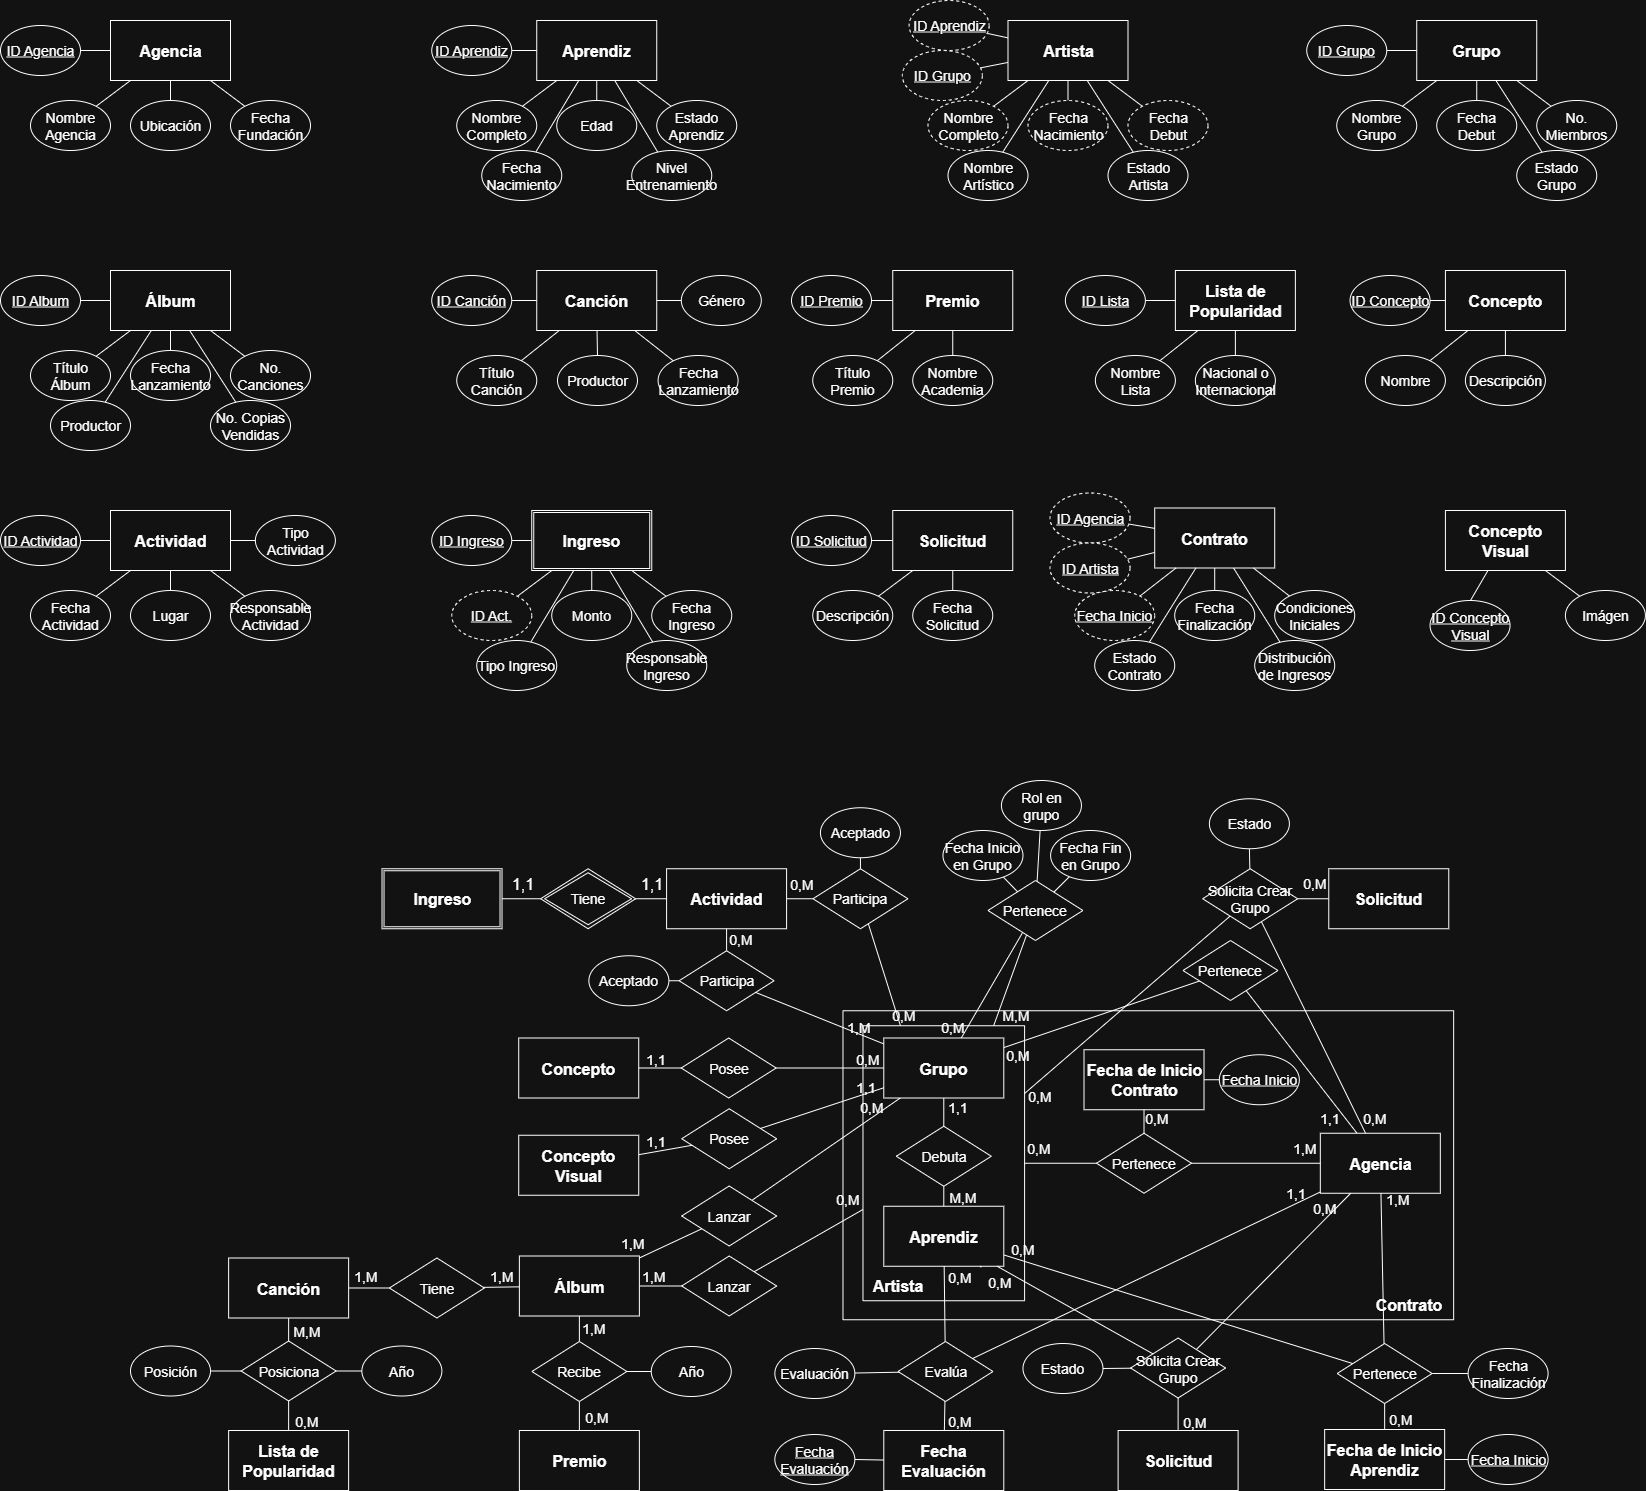
\includegraphics[width=1\textwidth]{merx.png}
\caption{Modelo Entidad–Relación Extendido (MERX) del Sistema K-POP World}
\end{figure}

\chapter{Solución Propuesta}
El modelo conceptual definido mediante el Modelo Entidad–Relación Extendido sirvió
como base directa para la implementación del sistema, garantizando la correspondencia
entre el diseño del dominio y la solución desarrollada.
La implementación se realizó utilizando PostgreSQL como sistema gestor de base de
datos, junto con Prisma como herramienta de mapeo objeto–relacional, lo que permitió
reflejar de forma estructurada las entidades, relaciones y restricciones definidas en el
modelo de datos.

\section{Organización Funcional del Sistema}
El sistema se organiza en módulos funcionales que agrupan responsabilidades relacionadas, facilitando la implementación y el mantenimiento del software. Cada módulo
interactúa con un subconjunto específico del modelo de datos, respetando las reglas y
restricciones definidas en el MERX y el diccionario de datos.
Esta organización modular se encuentra alineada con los principios de la arquitectura
limpia (Clean Architecture), promoviendo una clara separación entre la lógica de negocio
y los detalles de implementación.

\section{Justificación de la Solución Adoptada}
La solución propuesta permite modelar relaciones complejas, dependencias temporales y restricciones de integridad propias del dominio, garantizando la consistencia de la
información almacenada.
El uso de Clean Architecture, junto con PostgreSQL y Prisma, facilita la mantenibilidad del sistema y asegura que futuras modificaciones puedan realizarse sin comprometer
la coherencia del modelo de datos.

\chapter{Mantenimiento y Evolución del Sistema}
Esta sección presenta consideraciones técnicas orientadas al mantenimiento, extensión
y evolución futura del sistema de gestión de agencias y grupos de K-pop.

\section{Mantenibilidad}
El uso de una arquitectura limpia facilita el mantenimiento del sistema al separar
claramente la lógica de negocio de los detalles de implementación. Los cambios en la
interfaz de usuario o en la infraestructura de datos no afectan directamente al núcleo del
dominio, reduciendo el riesgo de errores.

\section{Escalabilidad}
La solución fue diseñada para soportar el crecimiento progresivo del sistema, tanto en
volumen de datos como en funcionalidades. PostgreSQL permite manejar grandes cantidades de información y relaciones complejas, mientras que Prisma facilita la gestión
eficiente de claves compuestas y consultas estructuradas.

\section{Extensión del sistema}
El sistema puede extenderse para incorporar nuevas funcionalidades, tales como la
gestión de giras internacionales, la integración con plataformas de streaming musical, el
análisis estadístico de popularidad y la generación de reportes financieros avanzados.
Estas extensiones pueden implementarse respetando las capas de la arquitectura, sin
modificar las reglas centrales del dominio.

\section{Buenas Prácticas de Desarrollo}
Para garantizar la calidad y estabilidad del sistema, se recomienda:
\begin{itemize}
    \item Mantener la separación de responsabilidades entre capas.
    \item Documentar adecuadamente los cambios realizados.
    \item Implementar pruebas unitarias sobre la capa de dominio.
    \item Validar reglas de negocio en la capa de aplicación.
    \item Utilizar migraciones controladas para cambios en la base de datos.
\end{itemize}

\chapter{Conclusiones}
El desarrollo del sistema de gestión de agencias y grupos de K-pop permitió abordar
un dominio complejo mediante un modelo de datos estructurado y coherente, capaz de
representar relaciones dinámicas, temporales y contractuales.
La definición del diccionario de datos y del Modelo Entidad–Relación Extendido ase-
gura la consistencia entre el diseño conceptual y la implementación, mientras que el uso
de una arquitectura limpia favorece la mantenibilidad y evolución del sistema.
En conjunto, la solución propuesta constituye una base sólida para la gestión de la
información del dominio y para la incorporación de futuras funcionalidades, manteniendo
la integridad y coherencia de los datos.
\end{document}